\chapter{Processing video}
In this section we'll show you how to deal with videos using OpenIMAJ. We provide a 
set of tools for loading, displaying and processing various kinds of video. 

All videos in OpenIMAJ are subtypes of the \verb+Video+ class. This class is typed 
on the type of underlying frame. In this case, let's create a video which holds coloured frames:
\begin{lstlisting}[language=java]
Video<MBFImage> video;
\end{lstlisting}

Exactly what kind of video is loaded depends on what you want to do. To load a video from a file
we use the \textbf{Xuggle} library which internally uses \verb+ffmpeg+. Let's load a video 
from a file (which you can download from here: \url{http://dl.dropbox.com/u/8705593/keyboardcat.flv}).

First you'll need to install Xuggle. Go to http://www.xuggle.com/xuggler/downloads/ and pick your platform 
then follow the instructions.

While this is downloading, let's write the code.
\marginpar{The \texttt{XuggleVideo} class also has a constructor that lets you pass a URL to a video on the web without downloading it first.}
If we want to load a video from a file we use a \verb+XuggleVideo+ object: 
\begin{lstlisting}[language=java]
video = new XuggleVideo(new File("/path/to/keyboardcat.flv"));
\end{lstlisting}

If your computer has a webcam, OpenIMAJ also supports live video input. These are called capture 
devices and you can use one through the \verb+VideoCapture+ class:
\begin{lstlisting}[language=java]
video = new VideoCapture(320,240);
\end{lstlisting}
This will find the first video capture device attached to your system and render it as closely to 
$320\times240$ pixels as it can. To select a specific device you can use the alternative constructors
and use the \verb+VideoCapture.getVideoDevices()+ static method to obtain the available devices.

Note that webcam capture does not require a Xuggle install and is completely built into OpenIMAJ.

To see if either of these kinds of video work, we can use \verb+VideoDisplay+ to display videos. This is 
achieved using the static function calls in \verb+VideoDisplay+ (which mirror those found in 
\verb+DisplayUtilities+ for images) like so:
\begin{lstlisting}[language=java]
VideoDisplay<MBFImage> display = VideoDisplay.createVideoDisplay(video);
\end{lstlisting}

Simply by creating a display, the video starts and plays. You can test this by running 
your app after Xuggle is installed. 
\marginpar{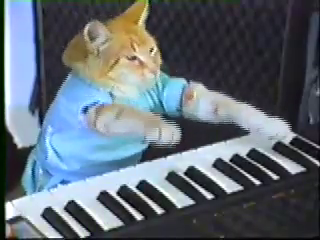
\includegraphics[width=\marginparwidth]{frame.png}}

\textbf{Note:} If you're using Linux or MacOSX, you might encounter an error trying to run this from Eclipse. 
This is due to library dependencies on Xuggle. To fix this, in Eclipse go to the run configuration 
(\verb+Run>Run Configurations+). Once here click the \verb+Environments+ tab. Add a new environment 
variable called \verb+DYLD_LIBRARY_PATH+ on MacOSX or \verb+LD_LIBRARY_PATH+ on Linux and set this to 
the location of the \verb+xuggler/lib+ directory (this is likely to be \verb+/usr/local/xuggler/lib+
if you went with the default Xuggle install options).

As with images, displaying them is nice but what we really want to do is process the frames of 
the video in some way. This can be achieved in various ways; firstly videos are \verb+Iterable+, so you can 
do something like this to iterate through every frame and process it:
\begin{lstlisting}[language=java]
for (MBFImage mbfImage : video) {
    DisplayUtilities.displayName(mbfImage.process(new CannyEdgeDetector2()), "videoFrames");
}
\end{lstlisting}
Here we're applying a Canny edge detector to each frame and displaying the frame in a named window. Another 
approach, which ties processing to image display automatically, is to use an event driven technique:
\marginpar{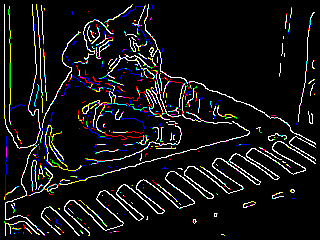
\includegraphics[width=\marginparwidth]{frame-canny.png}}
\begin{lstlisting}[language=java]
VideoDisplay<MBFImage> display = VideoDisplay.createVideoDisplay(video);
display.addVideoListener(
  new VideoDisplayListener<MBFImage>() {
    @Override
    public void beforeUpdate(MBFImage frame) {
        frame.processInplace(new CannyEdgeDetector2());
    }

    @Override
    public void afterUpdate(VideoDisplay<MBFImage> display) {
    }
  });
\end{lstlisting}

These \verb+VideoDisplayListener+s are given video frames before they are rendered and they are handed the 
video display after the render has occurred. The benefit of this approach is that functionality such as 
looping, pausing and stopping the video is given to you for free by the \verb+VideoDisplay+ class. 

\section*{Exercises}
\subsection*{Exercise 1: Applying different types of image processing to the video}
Try a different processing operation and see how it affects the frames of your video.
